\documentclass[12pt,a4paper]{article} %scrbook}%bookof}



% makes nice font


%fills A4 page
\usepackage{a4wide}
\usepackage[inner=2cm,outer=2cm, bottom = 2.0cm]{geometry}   %nice setting for twoside binding



%\usepackage[utf8]{inputenc}   % damit man Umlaute direkt eingeben kann und diese erkannt werden.
\usepackage[T1]{fontenc}        % Umlaute werden als eine Einheit angesehen -> richtige Trennung;
% ausserdem: die T1-Fonts gibt es auch in
% größeren Größen
%\usepackage{ae,aecompl}
\usepackage{units}
\usepackage[english]{babel}      %hiermit erhält man z.B. 'Abb.' statt 'Fig.' bei Bildbeschriftungen
\usepackage[utf8]{inputenc}
%\makeglossary                   % zwischendurch makeindex disseration aufrufen
\usepackage{enumerate}
\usepackage{latexsym}


%\clearscrplain
%\clearscrheadings

\usepackage[headsepline]{scrlayer-scrpage}
%\usepackage[]{scrpage2}
%\clearplainofpairofpagestyles
%\clearscrheadings
\pagestyle{scrheadings}

\cofoot[\pagemark]{\pagemark}% optionales Argument --> plain
%\clearscrheadings
\rohead{NAWI Graz}
\chead{
	Exercise Statistical Physics \\{\small Contact: gerhard.dorn@tugraz.at}}
\lohead{ITP}
\usepackage{titlesec}
\titleformat{\section}
{\normalfont\large\bfseries}{\thesection}{1em}{}


\usepackage{amsmath,amsthm,amsfonts}
%\usepackage{showkeys}
%\usepackage{epsfig}
%\usepackage{epic}
\usepackage{xr}

\usepackage{graphicx}
%\usepackage{inmthesis}
\usepackage{hyperref}
\usepackage{verbatim}
\usepackage[sorting=none, hyperref=true, backref=true]{biblatex}
\addbibresource{./library.bib}
%boxes
\usepackage{mdframed}
\usepackage{tensor}
%unity operator
%\usepackage{bbold}

 \setcounter{section}{3}
\begin{document}

 %\begin{center}
 %Technische Universität Graz \\
 %Institut für Theoretische Physik - computational physics \\
 %Prof. Dr. Wolfgang von der Linden \\
 %Kontakt: gerhard.dorn@tugraz.at
 %\end{center}
 
 
 \vspace{1cm}
 
 \section{Volume of a $d$-dimensional sphere}
\begin{itemize}
\item[a)] Calculate the volume $V_d(R)$ of a $d$-dimensional sphere with radius $R$. 
To do that write down the $d$-dimensional spherical coordinates and express the searched integral in those. 
In order to derive an expression for the $d$-dimensional spatial angle $\Omega_d$ examine the $d$-dimensional Gauß-integral. Show that
\begin{align}
\int_{-\infty}^\infty \dots \int_{-\infty}^\infty e^{-\vec{x}^2} d^dx = \left(\int_{-\infty}^\infty e^{-x^2}dx\right)^d = \pi^{d/2}
\end{align} and use its represenation in spherical coordinates to derive the spherical angle $\Omega_d$.

\item[b)] Pealing a multidimensional orange does not make sense. Argue why! Given is a $d$-dimensional orange with radius $R$. At which dimension $d$ is the volume of an outer shell of the orange with a thickness of $R\cdot 10^{-6}$ a million times bigger than the volume of the inner fruit?
\end{itemize} 

\begin{figure}[h!]
\begin{center}
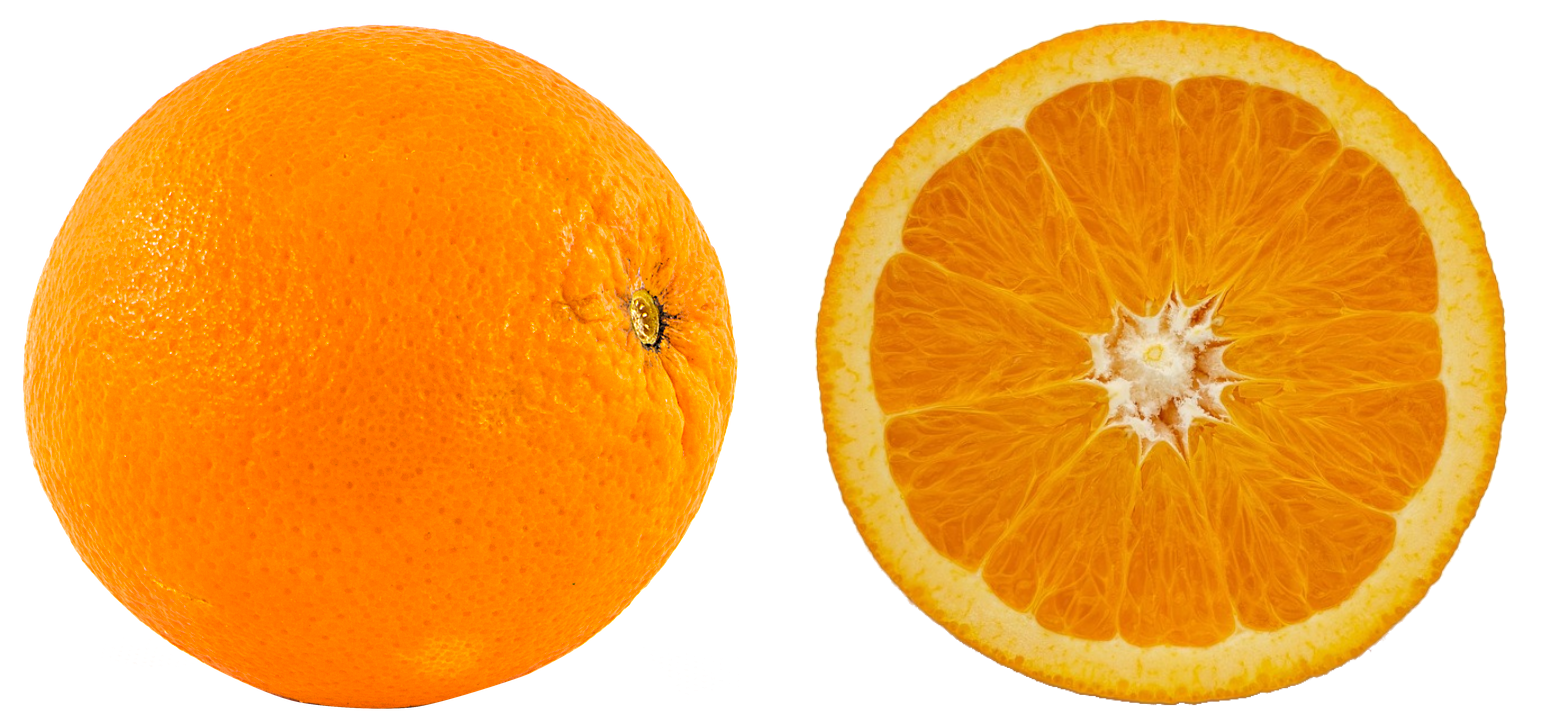
\includegraphics[width= 0.7\textwidth]{oranges.png} 
\caption[Sketch of a multidimensional orange]{Sketch of a multidimensional orange ($d=3$)\footnotemark.}  
\end{center}
\end{figure}

 \section{Ideal gas - phase space}
 Given is an ideal gas\footnote{Particles of an ideal gas are infinitely small (no collisions) and do not interact with each other (no attraction, no van der Waals force, etc.). Compare this concept with the generalization of a real gas (van der Waals gas equation).} with $N$ identical, classical particles with the particle mass $m$ which are confined in a square box of volume $V$.
 Each particle is characterized by its position $\boldsymbol{x}$ and momentum $\boldsymbol{p}$. No external potential (like gravity or electric field) is applied.
 
 \begin{itemize}
  \item What is a proper description of a microstate of such a particle? How many degrees of freedom are there?
 \end{itemize}
 We want to fix another quantity namely the total energy $E$.
 \begin{itemize}
  \item What does this restriction imply on the counting of microstates? How can you relate the total fixed energy $E$ to the characterization of microstates? (Just calculate the total energy of a given microstate.).
 \item Write down the expression for the partition sum $Z(N,V,E)$. How are discrete ($N$) and continuous scales ($V,E$) are considered?
 \end{itemize}
 
Since the condition $E_{\textnormal{microstate}} = E$ is hard to evaluate for a continuous variable we use a trick. 
Similar to the condition for the volume where the position of all microstates has to be within the volume, we want to count all microstates that have a lower energy than $E$ using the condition $E_{\textnormal{microstate}} \leq E$. We call this quantity volume of the phase space\footnote{Try to explain the name.} $F(N,V,E)$
$$F(N,V,E) := \int_0^E Z(N,V,E') dE'$$ and recognise that
\begin{align} 
Z(N,V,E) = \frac{\partial }{\partial E}  F(N,V,E).
\end{align}

 \begin{itemize}
  \item Use the result for the $n$--dimensional sphere to evaluate $F(N,V,E)$ and calculate $Z(N,V,E)$. Keep terms of order $N$ or higher. Recall the result of Problem~4 of the multidimensional orange. How could you relate $F$ and $Z$?
  \item Calculate the entropy $S(N,V,E)$ of the ideal gas in the box.
 \end{itemize}
 
 \section{Gibb's paradox}
 Now assume we have one box which is seperated in two volumes $V_1$ and $V_2$ which are separated by a virtual wall. The particles can move freely in the whole box which shall be in equilibrium, so the entropy is maximal which is realized by having equal particle densities in two virtual volumes\footnote{You can imagine the process as follows: Having the whole box in equilibrium take a snapshot of the system and count how many particles $N_i$ are in which virtual volume $V_i$.} $\frac{N_1}{V_1} = \frac{N_2}{V_2} =: n$ (for the proof see lecture notes Ch.~1.2.2). Since the densities are the same the average energy per particle is also the same $\frac{E_1}{N_1} = \frac{E_2}{N_2} =: \tilde{E}$.
 
 From the lecture we know, that the total entropy of the system should be equal to the sum of the two virtual volumes (it should not make a difference how we combine microstates). Entropy as such should be an extrinsic quantity and as such additive. We want to check this now:
 \begin{itemize}
  \item Calculate the individual entropies $S_1(N_1,V_1, E_1)$, $S_2(N_2,V_2,E_2)$ and the total entropy $S(N_1+N_2, V_1+V_2, E_1 + E_2)$ and express $\Delta S = S - S_1 - S_2$.
  \item Is the entropy increasing or decreasing when mixing those identical particles?
 \end{itemize}
 Experiments show that when mixing identical particles the entropy is not increasing. Theory tells us that the demanded additivity of entropy is violated. This result not gaining the same entropy is called \textbf{Gibbs paradox}.
 \paragraph{Quantum correction:} One solution to this paradox can be given by quantum physics. Claiming that gas particles are indistinguishable will lead to an extra term that leads to an extensive entropy.
 \begin{itemize}
  \item Reformulate $Z(N,V,E)$ and $S(N,V,E)$ for indistinguishable particles and show that entropy is extensive: 
  $$S(\alpha N, \alpha V, \alpha E) = \alpha S(N,V,E) .$$ 
 \end{itemize}
Another import consequence from quantum physics is \textbf{Heisenberg's uncertainty principle} which states that position and momentum cannot be measured at the same time\footnote{When evaluating entropy which is proportional ot the logarithm of number of microstates a particle can have, for a continuous scale, it diverges. Before quantizing phase space physicists used regularization techniques to overcome these singularities.}. The uncertainty is quantified by $ \Delta x \Delta p \geq h$ \footnote{With Planck's constant $h = 6.62607015 \times 10^{-34}$J / Hz (since 20th of May 2019 exact value).} and gives the minimal phase space volume one can resolve. Therefore it is reasonable to divide the whole $6N$ dimensional phase space volume by $h^{3N}$.

This principle comes into play when calculating the phase space.
\begin{itemize}
 \item Use the quantum correction and the discretization of phase space to derive the entropy $S(N,V,E)$ for the ideal gas. (Keep terms of the order $N$)
\end{itemize}
 This equation is referred to as \textbf{Sackur-Tetrode equation}.\\
Compare with the lecture notes (p. 87).\\[1cm]

\paragraph{Mixing entropy of different gases:} Assume the two volumes $V_1$ and $V_2$ contain two different gases (e.g. Helium and Neon) which are separated by a wall in the beginning. The densities shall be the same (equal presure in both volumes).
\begin{itemize}
 \item Calculate the mixing entropy when removing this wall using the correct quantum corrections.
\end{itemize}




 
 
% \printbibliography
 
 
 
 \vspace{2cm}
 \begin{minipage}[t]{1\textwidth}
 	\raggedleft
 	\centering
 	
\includegraphics[width = 0.20\textwidth]{CC-BY_icon}
 	\vspace{0.2cm}
 	
 	\centering
 	{\Large Gerhard Dorn} \\
 	https://creativecommons.org/licenses/by/4.0/legalcode
 \end{minipage}


  \end{document}
  
  
